\documentclass[border=2pt]{standalone}
\usepackage{diagrams}
\usetikzlibrary{patterns,angles,quotes,arrows.meta,math,calc}
\usepackage{amsmath}
\tikzset{
  edge/.style={line width=1pt},
  vlbl/.style={font=\normalsize},
  elbl/.style={font=\small},
  dotnode/.style={circle, fill=black, inner sep=2pt},
}
\begin{document}
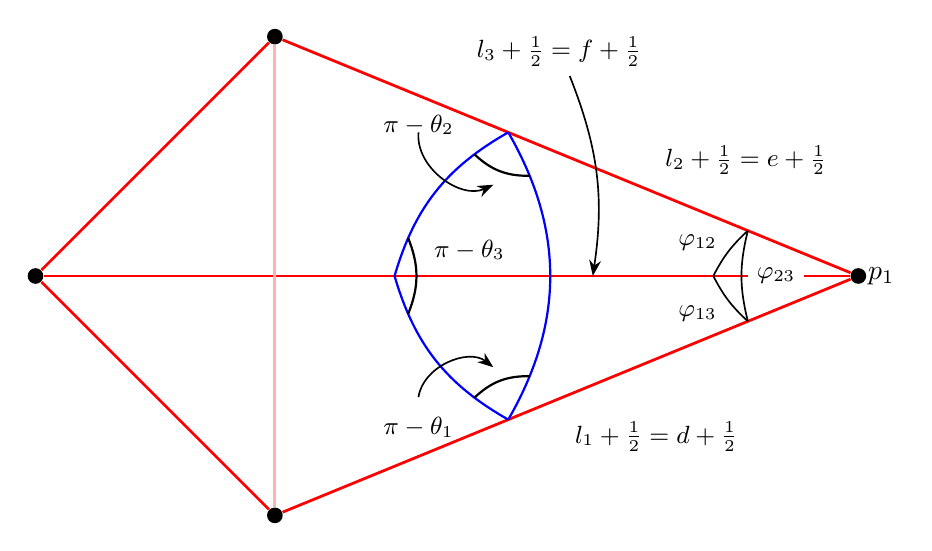
\begin{tikzpicture}[scale=0.95]
  \node[dotnode]  (Al) at (-5, 0) {};      % far left vertex
  \node[dotnode]  (At) at (-1.8, 3.2) {};  % top vertex
  \node[dotnode]  (Ab) at (-1.8,-3.2) {};  % bottom vertex
  \node[dotnode]  (p1) at ( 6, 0) {};      % right apex

  % outer kite / tetrahedron seen edge-on
  \draw[edge,color=red] (Al)--(At)--(p1)--(Ab)--(Al);
  \draw[edge,color=red] (Al)--(p1);           % horizontal axis (edge p1--Al)
  \draw[edge,color=red!30] (At)--(Ab);           % horizontal axis (edge p1--Al)

  % points where the small sphere around p1 meets the three edges to At,Ab,Al
  \coordinate (Vu) at ($(p1)!0.60!(At)$);
  \coordinate (Vl) at ($(p1)!0.60!(Ab)$);
  \coordinate (Vm) at (-0.2,0);      % on the axis, left vertex of spherical triangle

  % straight meridians p1 -> vertices (already partly along kite edges/axis)
  % spherical-triangle edges (arcs)
  \draw[line width=0.8pt,color=blue] (Vu) to[bend right=22] node[pos=0.2] (au1) {}node[pos=0.8] (am1) {}  (Vm);   % upper-left edge
  \draw[line width=0.8pt,color=blue] (Vm) to[bend right=22]  node[pos=0.2] (am2) {}  node[pos=0.8] (al1) {} (Vl);   % lower-left edge
  \draw[line width=0.8pt,color=blue] (Vu) to[bend left=30] node[pos=0.15] (au2) {} node[pos=0.85] (al2) {}  (Vl);   % right edge (bulges toward p1)
\draw[line width=0.8pt] (au1.center) to[bend right=22] (au2.center);
\draw[line width=0.8pt] (al1.center) to[bend left=22] (al2.center);
\draw[line width=0.8pt] (am1.center) to[bend left=22] (am2.center);

  % small angle arcs at p1 (phi_ik between the three meridians)
  \path (p1) -- (Vu) coordinate[pos=0.3] (u1);
  \path (p1) -- (Vl) coordinate[pos=0.3] (l1);
  \path (p1) -- (Vm) coordinate[pos=0.30] (m1);
  \path (p1) -- (Vu) coordinate[pos=0.40] (u2);
  \path (p1) -- (Vl) coordinate[pos=0.40] (l2);
  \draw[line width=0.6pt] (u1) to[bend right=10] (m1);   % phi_12
  \draw[line width=0.6pt] (m1) to[bend right=10] (l1);   % phi_13
  \draw[line width=0.6pt] (u1) to[bend right=14]  (l1);   % phi_23 (wider)

  % phi labels near p1
  \node[elbl] at (3.85, 0.45) {$\varphi_{12}$};
  \node[elbl] at (3.85,-0.50) {$\varphi_{13}$};
  \node[elbl,fill=white] at (4.9, 0) {$\varphi_{23}$};

  % spherical-triangle vertex (dihedral) angles pi - theta_i
  \draw[-{Stealth[length=2mm]},line width=0.6pt]  ($(Vu)+(-1.2,0)$) to[bend right=60]  ($(Vu)+(-0.2,-0.7)$);
  \node[elbl] at ($(Vu)+(-1.2,0.1)$) {$\pi-\theta_2$};
  \node[elbl] at ($(Vm)+(1.0,0.35)$) {$\pi-\theta_3$};
   \draw[-{Stealth[length=2mm]},line width=0.6pt]  ($(Vl)+(-1.2,0.3)$) to[bend left=60]  ($(Vl)+(-0.2,0.7)$);
  \node[elbl] at ($(Vl)+(-1.2,-0.1)$) {$\pi-\theta_1$};

  % edge (l_i) labels with pointer arrows
  \node[elbl] (Lf) at (2, 3) {$l_3+\tfrac12=f+\tfrac12$};
  \draw[-{Stealth[length=2mm]},line width=0.6pt] (Lf) to[bend left=15] (2.45,0);
  \node[elbl] at (4.5, 1.55) {$l_2+\tfrac12=e+\tfrac12$};
  \node[elbl] at (3.3,-2.15) {$l_1+\tfrac12=d+\tfrac12$};

  \node[vlbl,right] at (p1) {$p_1$};
\end{tikzpicture}
\end{document}